
%(BEGIN_QUESTION)
% Copyright 2008, Tony R. Kuphaldt, released under the Creative Commons Attribution License (v 1.0)
% This means you may do almost anything with this work of mine, so long as you give me proper credit

Use Kirchhoff's Voltage Law to calculate the magnitude and polarity of the voltage across resistor $R_4$ in this resistor network.  You must sketch polarity marks (+ , -) on the schematic diagram to show the polarity of $V_{R4}$, as well as show all of your mathematical work!

$$\includegraphics[width=15.5cm]{i02526x01.eps}$$

\vfil 

\underbar{file i02526}
\eject
%(END_QUESTION)





%(BEGIN_ANSWER)

This is a graded question -- no answers or hints given!

%(END_ANSWER)





%(BEGIN_NOTES)

$$\includegraphics[width=15.5cm]{i02526x02.eps}$$

%INDEX% Electronics review: Kirchhoff's Voltage Law (KVL)

%(END_NOTES)


